\section{Robustness Analysis}

\subsection{Generalization ability}

In this section we will focus on the generlization of the model,
that is to test model on irrelevant player or match.
The model is trained on first 16 matches and test on the rest matches.

\paragraph{Prediction of Other Matches}~{}

A figure of swing difference on train match, and a figure of swing difference on test match are displayed.

\begin{figure}[H]
    \centering
    \begin{subfigure}[b]{0.5\textwidth}
        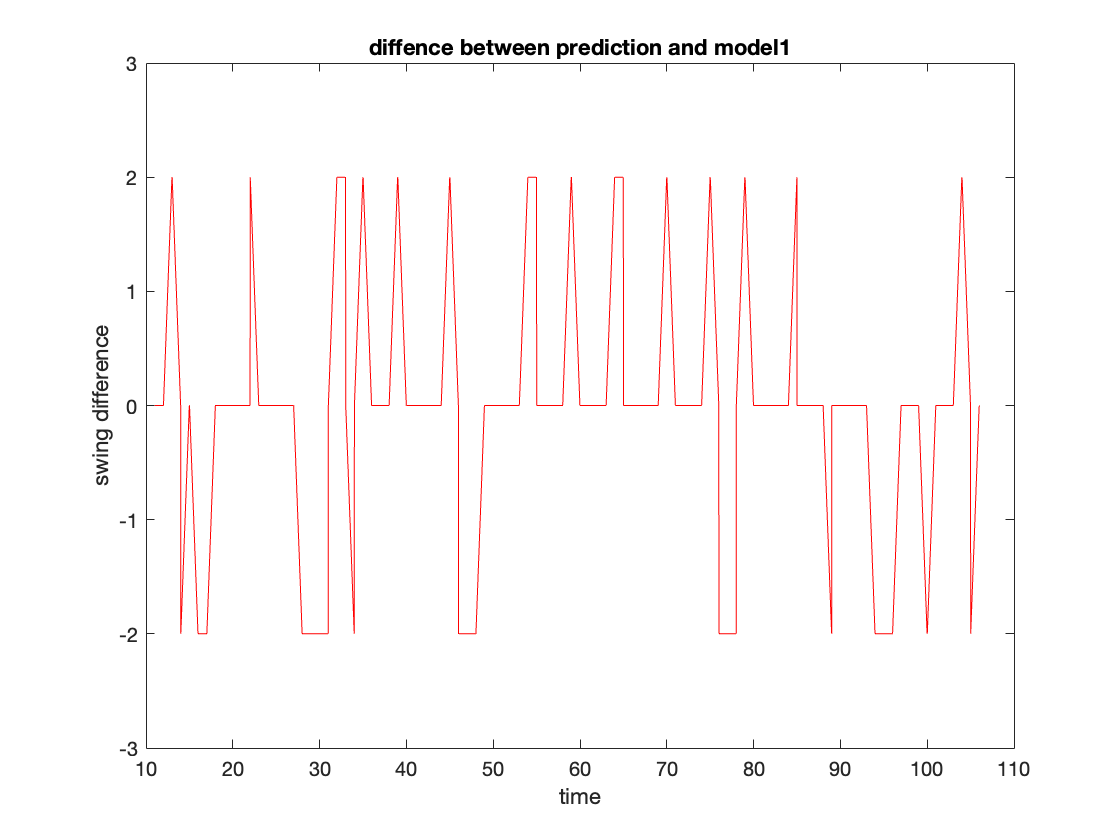
\includegraphics[width=\linewidth]{mainmatter/imgs/generalization_train.png}
        \caption{train match}
    \end{subfigure}\hspace{-0.02\textwidth}
    \begin{subfigure}[b]{0.5\textwidth}
        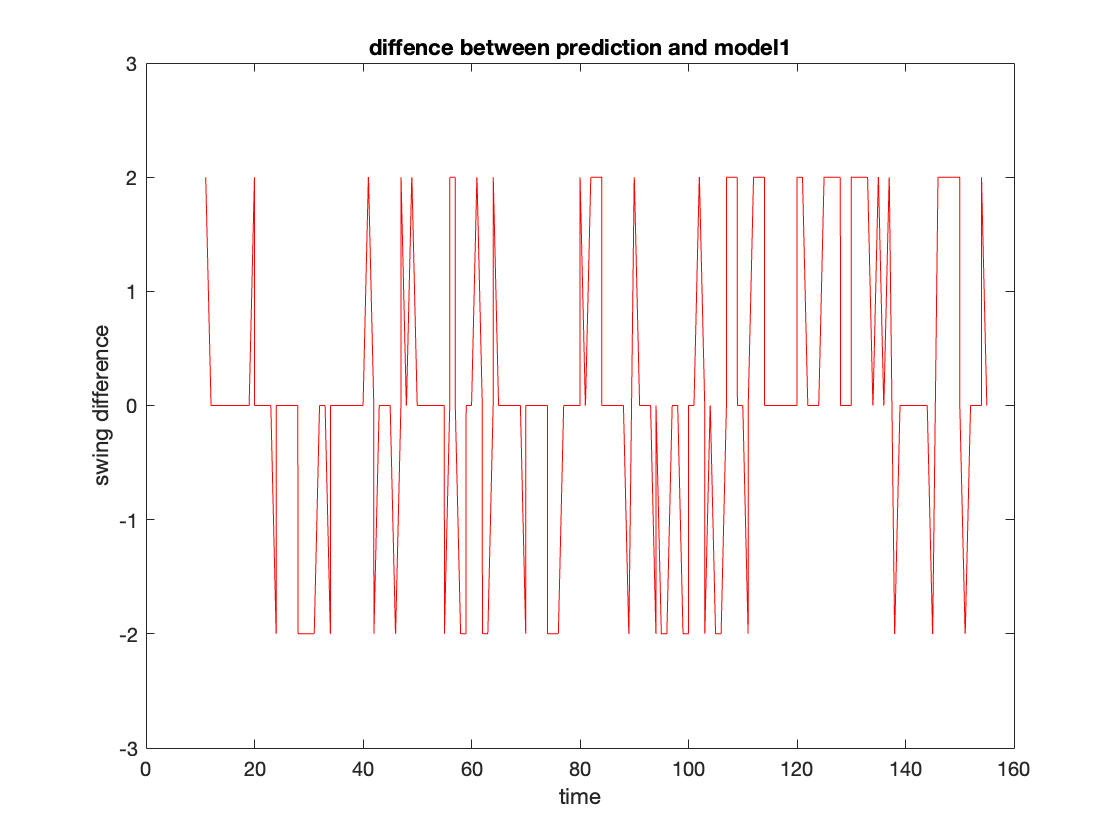
\includegraphics[width=\linewidth]{mainmatter/imgs/generalization_test.png}
        \caption{test match}
    \end{subfigure}\hspace{-0.02\textwidth}
    \caption{difference on train and test match}
    \label{fig:generalization}
\end{figure}

Table of accuracy on train and test match is displayed.

\begin{table}[H]
    \centering
    \begin{tabular}{cccccc}
        \toprule
        \textbf{Step} & \textbf{1} & \textbf{2} & \textbf{3} & \textbf{4} & \textbf{5} \\
        \midrule
        \textbf{Train Set} & 0.4495 & 0.4426 & 0.4374 & 0.4370 & 0.4250 \\
        \textbf{Test Set} & 0.4115 & 0.4016 & 0.3983 & 0.3994 & 0.3932 \\
        \bottomrule
    \end{tabular}
    \caption{Predict Rate for Each Step}
    \label{tab:predict_rate}
\end{table}

\paragraph{Analysis on Women's Tennis and Table Tennis}~{}

As for women's tennis, it is a pity that we did not find enough data online, but from all men's match predictions, the 
accuracy rate is stable, so we have every reason to believe that our data can also apply to women's matches. \\
For table tennis, technical statistics also includes: 
\begin{enumerate}
    \item more serve types, such as forehand, backhand, short, long, or sidespin serves.
    \item more receiving techniques,such as forehand push, backhand push, flick, or topspin.
\end{enumerate}
So we need to modify the influencing factors in our model, but the general framework is similar.

Now, we have finished Problem 4.

\subsection{Parameters Sensitivity Analysis}

Now we focus on the sensitivity of the first problem. We have to do this bacause the judgement of the parameters of 
influencing factors is subjective to some extent, so our result of parameters is a little different from reality. 
The function of momentum is a uniformly continuous function of parameters(because variables are normalized), so little
difference will not make the outcome of momentum imprecise.